\chapter{High Low Guessing Game With Hints}
\label{chapter:hlggwh}
\graphicspath{ {./Lab05HighLowWithHints/Fig} }



\section{Outcomes and Objectives}

The outcome of this lab is to modify existing code to add increased
functionality and instantiate it on oue development board.
Through this process you will achieve the following
learning objectives.
\begin{itemize}
	\itemsep=0em
	\item \Paste{bok:REP_WordStatement}
	\item \Paste{bok:REP_TruthTable}
\end{itemize}


\section{The Guessing Game with Hints}

This week's assignment asks you to add some enhanced functionality to
the guessing game. Since we are adding functionality to the guessing
game, it's worth reviewing the guessing game because we will use some of
the terms in the description of our enhanced functionality. The game
starts with the secret keeper generating a \emph{secret number} between
{[}0 and 15{]}, inclusive. Once the \emph{secret number} is decided, the
guesser makes a \emph{guess}, a number in the interval {[}0 to 15{]}
inclusive, and tells this to the secret keeper. The secret keep then
replies to the guesser if \emph{guess} is less than, equal to, or
greater than the \emph{secret number}. The game continues with repeated
guesser/secret keeper exchange until the guesser correctly identifies
the \emph{secret number}.

In this week's assignment, you will add circuitry to provide an
indication of how far the user's guess is from the secret number by
telling them if their \emph{guess} is hot (close to the \emph{secret
number}), warm (kind-of close to the \emph{secret number}), or cold (far
away from the \emph{secret number}).

The user input and output, shown in Figure~\ref{fig:iOonDevBorad} are the same as last week's
assignment with the exception of the \textbf{hotCold} button and
\textbf{clue} 7-segment display.

\begin{figure}[ht]
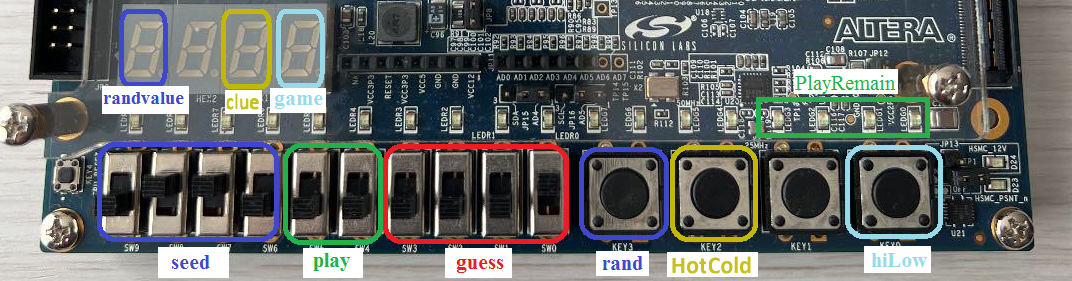
\includegraphics[width=0.8\paperwidth]{ image1.png}
\caption{The input and output you should use to realize your digital system.}
\label{fig:iOonDevBorad}
\end{figure}

The functionality of the inputs and outputs from last week's assignment
are unchanged; the \textbf{hotCold} button and \textbf{clue} 7-segment
display operate as follows.

The player can request a more refined evaluation of their guess by
pressing the \textbf{hotCold} button. To make this evaluation, the
absolute value of the difference between the \emph{guess} and
\emph{secret number} is computed and then comapred against warmThreshold
and coldThreshold as shown in Figure~\ref{fig:guessThreshold}.

\begin{itemize}
\item
  If difference \textless{} warmThreshold the guess is Hot
\item
  If (difference \textgreater= warmThreshold) and (difference
  \textless{} coldThreshold) the guess is Warm
\item
  If difference \textgreater= coldThreshold the guess is Cold
\end{itemize}

\begin{figure}[ht]
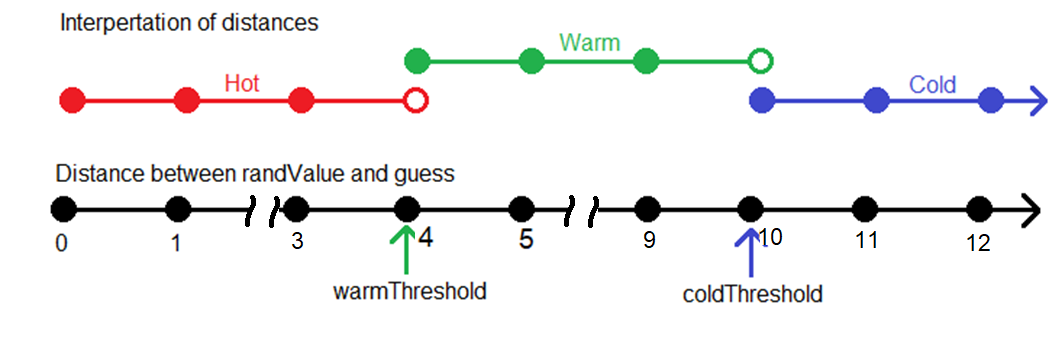
\includegraphics{ image2.png}
\caption{The interpretation of the quality of a guess in terms of thresholds.}
\label{fig:guessThreshold}
\end{figure}

The difference is always a positive number. For example, if the user's
\emph{guess} was 43 and the secret number was 45, then the difference
would be 2 making this guess Hot (according to Figure~\ref{fig:guessThreshold}). If
\emph{guess} was 45 and the \emph{secret number} was 43, the difference
would be 2 and this guess would also be Hot. Explore the relationship
between guess, secret number and the Quality of the guess by completing
Table~\ref{table:applyGuessIntervals}.

\begin{longtable}[]{@{}
|  >{\raggedright\arraybackslash}p{(\columnwidth - 6\tabcolsep) * \real{0.2499}}|
  >{\raggedright\arraybackslash}p{(\columnwidth - 6\tabcolsep) * \real{0.2499}}|
  >{\raggedright\arraybackslash}p{(\columnwidth - 6\tabcolsep) * \real{0.2501}}|
  >{\raggedright\arraybackslash}p{(\columnwidth - 6\tabcolsep) * \real{0.2501}}|@{}}
\caption{Determine the quality of a guess at the secret number.
Your answer may be a number, pair of numbers, a range or a pair of
ranges. Assume a 4-bit word size for guess and the secret number and
warmThreshold = 4 and ColdThreshold=10.}
\label{table:applyGuessIntervals}
\tabularnewline
\toprule()
\begin{minipage}[b]{\linewidth}\raggedright
\emph{guess}
\end{minipage} & \begin{minipage}[b]{\linewidth}\raggedright
\emph{secret number}
\end{minipage} & \begin{minipage}[b]{\linewidth}\raggedright
difference
\end{minipage} & \begin{minipage}[b]{\linewidth}\raggedright
Quality
\end{minipage} \\
\midrule()
\endfirsthead
\toprule()
\begin{minipage}[b]{\linewidth}\raggedright
\emph{guess}
\end{minipage} & \begin{minipage}[b]{\linewidth}\raggedright
\emph{secret number}
\end{minipage} & \begin{minipage}[b]{\linewidth}\raggedright
difference
\end{minipage} & \begin{minipage}[b]{\linewidth}\raggedright
Quality
\end{minipage} \\ 
\midrule()
\endhead
14 & 11 & & \\ \hline
8 & 12 & & \\ \hline
4 & 14 & & \\ \hline
8 & & 2 & Hot \\ \hline
& 8 & {[}4 to 9{]} & Warm \\ \hline
& 2 & {[}10 to 15{]} & Cold \\
\bottomrule()
\end{longtable}

The 7-segment display called clue will communicate the quality of the
user's guess to the user. It will do this by displaying `C' if the guess
is \textbf{\uline{C}}old, `A' if the guess is w\textbf{\uline{A}}rm, `H'
if the guess is \textbf{\uline{H}}ot.

\section{System Architecture}

There are an almost unlimited number of ways that you could implement
this digital system. For this lab, I want you to use the system
architecture shown in Figure~\ref{fig:guessWithHintSystemArch}. A few 
comments about the visual notation
used in this schematic are in order.

\begin{enumerate}
\def\labelenumi{\arabic{enumi})}
\item
  Lines with the same name are connected together.
\item
  When a signal is sent to multiple devices in close proximity, a grey
  line is used to show that the signal is ``underneath a device.
\item
  The input signals are color-coded to correspond to the colors used in
  Figure~\ref{fig:iOonDevBorad}.
\end{enumerate}

\begin{figure}[ht]
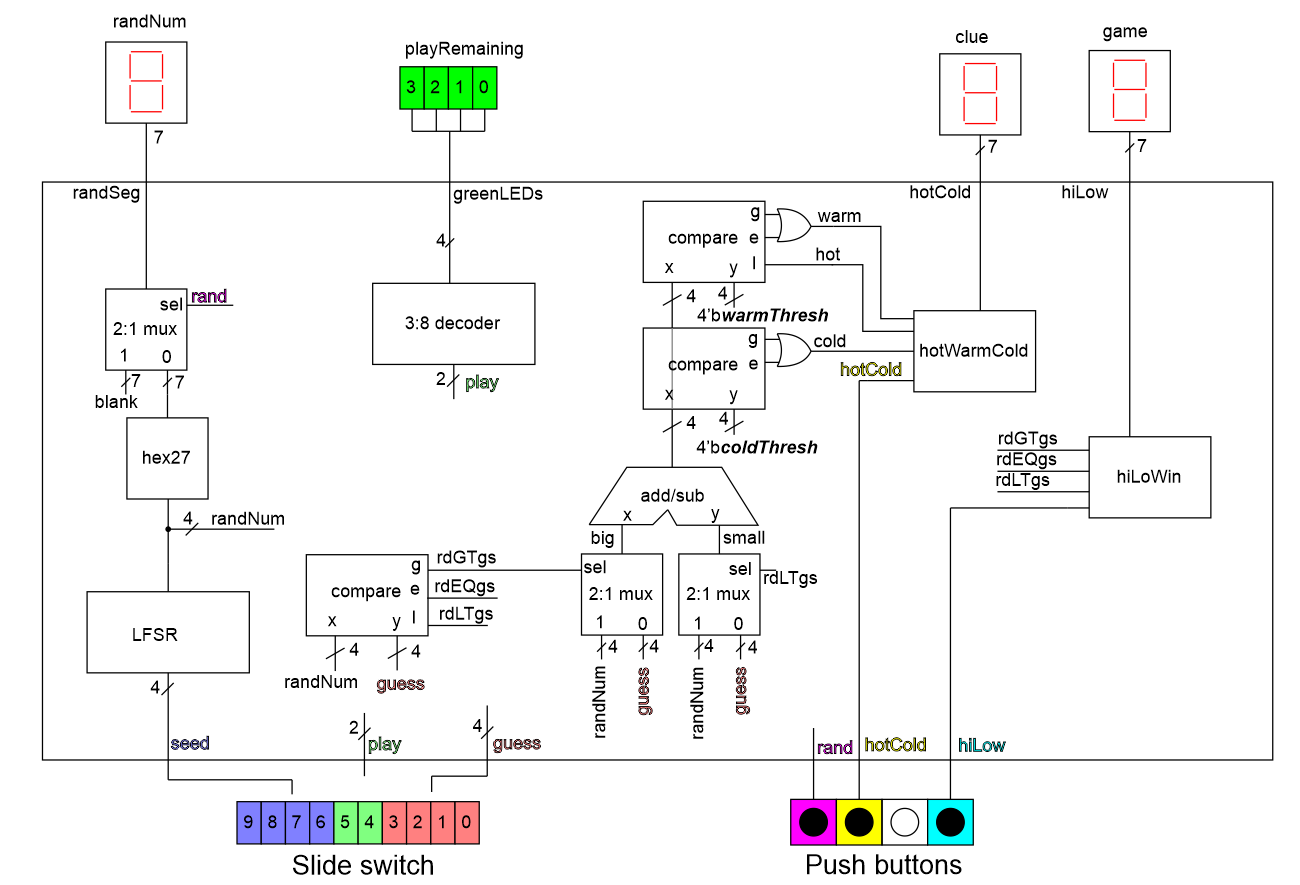
\includegraphics[width=6.50278in,height=4.42708in]{ image3.png}
\caption{System architecture for the guessing game with hint. The select
inputs on the big and small 2x1 muxes is intentionally not shown -- you
will need to figure this out.}
\label{fig:guessWithHintSystemArch}
\end{figure}

The new circuitry is shown in the middle of Figure~\ref{fig:guessWithHintSystemArch} starting with the
comparator whose inputs are \emph{randNum} and \emph{guess}. Actually,
this comparator should already be in your circuit because it provides
its outputs as the input to the hiLoWin module used in the previous lab.
This comparator is needed to determine the difference between
\emph{randNum} and \emph{guess} as follows.

The difference between the \emph{guess} and \emph{secret number} (called
\emph{randNum} in Figure~\ref{fig:guessWithHintSystemArch})that you computed 
in Table~\ref{table:applyGuessIntervals} is 
the absolute
value of the difference between \emph{guess} and the \emph{secret
number}. We will realize this functionality by placing the larger of
\emph{guess} or \emph{randNum} on the x input of the adder subtractor
shown in Figure~\ref{fig:guessWithHintSystemArch}. The smaller of \emph{guess} or \emph{randNum} is
placed on the y input of the adder subtractor. This routing of x and y
to the adder subtractor is performed by a pair of 4-bit 2x1 muxes whose
select inputs are controlled by one of the comparator's three outputs.
The adder subtractor in Figure~\ref{fig:guessWithHintSystemArch} is configured to subtract by hardwiring
its fnc input to 1'b1. You will need to determine which single output
from the comparator feeds the select input for this pair of muxes.

Let's call the output of the adder subtractor \emph{difference}. This
\emph{difference} is compared to the warmThreshold and coldThreshold
using a pair of comparators. The values of warmThresh and coldThresh are
set in code using the signal declaration and signal assignment
statements shown in Listing~\ref{listing:guessThresholds}.

\begin{lstlisting}[language=Verilog,
 caption={The signal declaration and assignment for guess thresholds.},
 label={listing:guessThresholds},
 frame=single]
    wire [3:0] warmThreshold, coldThreshold; 
    assign warmThreshold = 4'b0100;		
    assign coldThreshold = 4'b1010;
\end{lstlisting}

The output from the warmThreshold and coldThreshold comparators is used
as input to the hotWarmCold logic to display an appropriate character on
the \textbf{hotCold} 7-segment display. You will derive this logic as
you work through this lab.

\section{Module: 2:1 Mux}
This module was discussed in Lab 4.



\section{Module: Compare}
This module was discussed in Lab 4.


\section{Module: Add/Sub }

A N-bit adder subtractor is a basic building block in many digital
systems. The N-bit adder subtractor shown in Figure~\ref{fig:adderSubSymbol} adds 
its N-bit
input x and N-bit input y when fnc = 0 and places the result on the
N-bit output subDiff. When fnc = 1 the sumDiff output equals x-y. When
the inputs and output are interpreted as a 2's complement values, the
sovf output equals 1 when the computation results in an overflow. When
the inputs and output are interpreted as binary numbers, the uovf output
equals 1 when the computation results in an overflow.

\begin{figure}[ht]
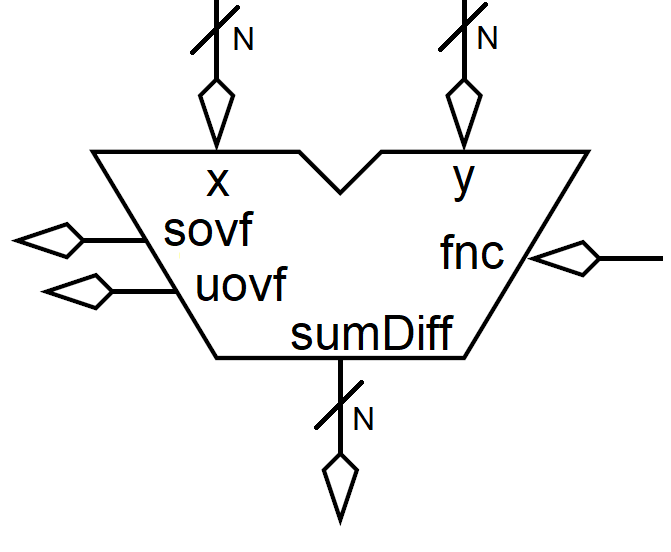
\includegraphics[width=0.3\paperwidth]{ image4.png}
\caption{A schematic representation of a N-bit adder subtractor.}
\label{fig:adderSubSymbol}
\end{figure}

I have provided you the Verilog code for the N-bit adder subtractor on
Canvas. This module instantiates N full-adders. Thus, you will need to
include the full adder module contained in the file fullAdder.v in your
project to instantiate a genericAdderSubtractor instance. Listing 2
shows the module declaration for the genericAdderSubtractor. Note that
the output from the module follows the fnc input. The module
instantiation shown in Listing 2 corresponds to the system architecture
shown in Figure~\ref{fig:guessWithHintSystemArch}. Since the inputs to the adder subtractor in the
system architecture will not generate overflow, the overflow outputs
from this adder subtractor are not needed. When you do not need an
output from a module, you can leave its parameter slot unfilled. This
explains the pair of empty fields at the end of the module instantiation
shown in Listing 2.

\begin{lstlisting}[language=Verilog,
 caption={Top, module definition for an adder subtractor.  Bottom, module instantation 
 of the adder subtractor in Figure~\ref{fig:guessWithHintSystemArch}.},
 label={listing:adderSubtractor},
 frame=single]
// Module definition for the comparator
module genericAdderSubtractor(a, b, fnc, sumDiff, sovf, uovf);

// Module instantiation for an adder subtractor in hiLow digital circuit
genericAdderSubtractor #(4) prox(big, small, 1'b1, difference, , );
\end{lstlisting}


Like the mux and comparator, the adder subtractor is a generic module.
This means that you need to specify the vector width of the \textbf{X}
and \textbf{Y} inputs and \textbf{sumDiff} output using the \#()
specifier. Pay close attention to match the value of this generic and
the size of the input and output vectors.


\section{Logic: hotWarmCold}

The goal of this section is to determine the logic inside the hotWarmCold logi blok
in Figure~\ref{fig:guessWithHintSystemArch}.  To do this you will first need to form three 
signals, \emph{hot}, \emph{warm}, and \emph{cold}.  These three signals describe how close the 
\emph{guess} is from \emph{randNum}. We will call the comparator that compares \emph{difference} 
and \emph{warmThresh}, the warm comparator and call its three outputs wGT, wEQ and wLT.
The other omprtor is the cold comparator nd its outputs preixed with  lowercase ``c''.

The warm and cold comparators generate a total of 6 signals, some of which are
sent to the logic block B1 and B2 to form the warm and cold signals - the logic for the
hot signal is given to you in Figure~\ref{fig:guessWithHintSystemArch}.

To understand the logic inside the B1 and B2 logic blocks let's look at an
example.  Use \emph{coldThresh} = 10 and \emph{warmThresh} = 4 to complete
Table~\ref{table:fillInCompareOperations}.  Do this by comparing the value in the column labeled
``\emph{difference}'' to \emph{warmThresh} and \emph{coldThresh} and
asserting the appropriate comparators outputs.  It may help for us to do one 
row together, \emph{difference} = 9. If we consider the
warm comparator, the x input equals 9 (the value of \emph{difference})
and the y input equals 4 (the value of \emph{warmThresh}). Since 9 is
greater than 4, the output wGT will equal 1 and wEQ and wLT will both
equal 0. If we consider the cold comparator, the x input equals 9 (the
value of \emph{difference}) and the y input equals 10 (the value of
\emph{coldThresh}). Since 9 is less than 10, the output cLT will equal 1
and cEQ and cGT will both equal 0. Finally, since \emph{difference}
equals 9 and this is between the warm and cold thresholds, the quality
of the guess should set warm = 1 and hot and cold to 0.

\begin{longtable}[]{@{}
| >{\raggedright\arraybackslash}p{(\columnwidth - 18\tabcolsep) * \real{0.1110}}|
  >{\raggedright\arraybackslash}p{(\columnwidth - 18\tabcolsep) * \real{0.1004}}|
  >{\raggedright\arraybackslash}p{(\columnwidth - 18\tabcolsep) * \real{0.1004}}|
  >{\raggedright\arraybackslash}p{(\columnwidth - 18\tabcolsep) * \real{0.1005}}|
  >{\raggedright\arraybackslash}p{(\columnwidth - 18\tabcolsep) * \real{0.1004}}|
  >{\raggedright\arraybackslash}p{(\columnwidth - 18\tabcolsep) * \real{0.1004}}|
  >{\raggedright\arraybackslash}p{(\columnwidth - 18\tabcolsep) * \real{0.1005}}|
  >{\raggedright\arraybackslash}p{(\columnwidth - 18\tabcolsep) * \real{0.0957}}|
  >{\raggedright\arraybackslash}p{(\columnwidth - 18\tabcolsep) * \real{0.0957}}|
  >{\raggedright\arraybackslash}p{(\columnwidth - 18\tabcolsep) * \real{0.0951}}@{}|}
\caption{Complete the following table to determine which
comparator outputs are needed to determine the quality of a guess. Let
warmThresh = 4 and coldThresh = 10.}\label{table:fillInCompareOperations}\tabularnewline
\toprule()
\multirow{2}{*}{difference} & 
	\multicolumn{3}{|c|}{warmThresh comparator} & 
	\multicolumn{3}{|c|}{coldThresh comparator} & 
	\multirow{2}{*}{Hot} &
	\multirow{2}{*}{Warm} & 
	\multirow{2}{*}{Cold} \\ \cline{2-7}
& wGT & wEQ & wLT & cGT & cEQ &  \\ \cline{2-7}
\midrule()
\endfirsthead
\toprule()
\multirow{2}{*}{difference} & 
	\multicolumn{3}{|c|}{warmThresh comparator} & 
	\multicolumn{3}{|c|}{coldThresh comparator} & 
	\multirow{2}{*}{Hot} &
	\multirow{2}{*}{Warm} & 
	\multirow{2}{*}{Cold} \\ \cline{2-7}
& wGT & wEQ & wLT & cGT & cEQ &  \\ \cline{2-7}
\midrule()
\endhead
3 & & & & & & & & & \\ \hline
4 & & & & & & & & & \\ \hline
5 & & & & & & & & & \\ \hline
9 & 1 & & & & & 1 & & 1 & \\ \hline
10 & & & & & & & & & \\ \hline
11 & & & & & & & & & \\
\bottomrule()
\end{longtable}

Now, you need to use the values in Table~\ref{table:fillInCompareOperations} to determine the logic for
each of the three outputs from the ``discrete logic'' block shown in
Figure~\ref{fig:guessWithHintSystemArch}. To do this, look at the conditions that cause each of the
outputs and write an expression using AND and OR to describe when that
output equals 1.  You 

\protect\hypertarget{hotWarmCold_Logic}{}{}
\begin{verbatim}
	Cold =                               // write logic description
	Warm =                            // write logic description
	Hot = wLT;                       // given to you in  Figure~\ref{fig:guessWithHintSystemArch}
\end{verbatim}

For the hotWarmCold block of code:

\begin{itemize}
\item
  Make three assign statements, one for hot, warm and cold
\item
  Use only \& and \textbar{} operations.
\item
  Use parenthesis to ensure proper order of operation.
\item
  The \emph{hot}, \emph{warm} and \emph{cold} signals should be ``wire''
  type.
\end{itemize}

You will implement the hotWarmCold logic using an always/case statement
that takes in as input the 3 outputs from the ``discrete Logic'' block,
\emph{hot}, \emph{warm} and \emph{cold}. These three outputs form a 1's
hot code because a guess can only be one of these three conditions at a
time. When the \textbf{hotCold} button is pressed, the output of the
hotWarmCold block forms an illuminate 7-segment representation of the
quality of the guess shown in Figure~\ref{figure:hiLoHintSevenSeg}. The 
7-segment output from the
hotWarmCold block should be blank when the \textbf{hotCold} button is
unpressed.

\begin{figure}[ht]
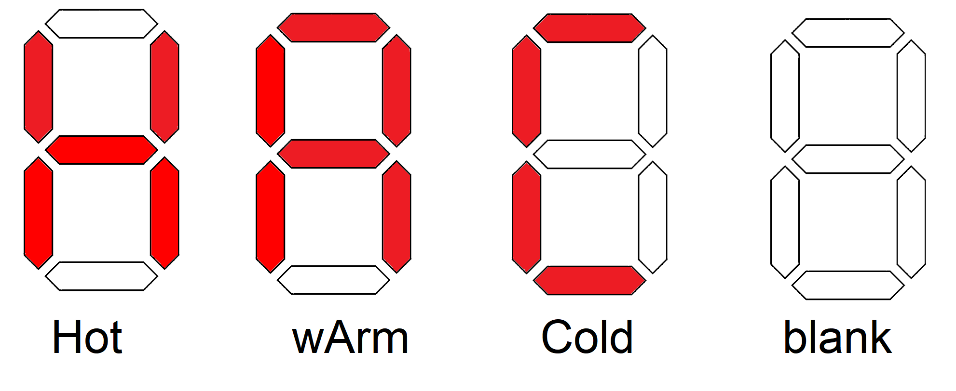
\includegraphics{ image5.png}
\caption{The illuminated patterns to inform the guesser about the magnitude of their guess.}
\label{figure:hiLoHintSevenSeg}
\end{figure}

For this block of code:

\begin{itemize}
\item
  Use an always/case statement.
\item
  Form a 4-bit vector from the \emph{hot}, \emph{warm}, \emph{cold}
  signals and the \textbf{hotCold} button.
\item
  Use this 4-bit vector as the input to the always/case statement.
\item
  Make sure that the output signal has ``reg'' type.
\item
  Include inline comments prior to the always/case statement describing
  the pattern that is displayed on the 7-segment display for each
  possible output. An example is given in Listing 3.
\end{itemize}

\begin{lstlisting}[language=Verilog,
 caption={A comment block describing the pattern of illuminated segment for each guess hint..},
 label={listing:hotColdGuess},
 frame=single]
//*********************************************
// Logic to display the quality of the guess
//	Hot  = `H' = <show binary code>
//	wArm = `A' = <show binary code>
//	Cold = `C' = <show binary code>
//
//		 hex[0]
//		 -----
//	hex[5]	|	|	hex[1]
//		|	|	
//		 -----	hex[6]
//	hex[4]	|	|
//		|	|	hex[2]
//		 -----
//		 hex[3]
//*********************************************
\end{lstlisting}


\section{Module: hiLow}
This is the top-level module in Figure~\ref{fig:guessWithHintSystemArch}, the outermost
block. \uline{If you were not able to get the previous lab working}, just
implement the functionality identified in this assignment and make the
\emph{randNum} come directly from the seed switch. In this case, you
should use the top module declaration in Listing~\ref{listing:hiLowModule}. If you got the
previous lab working correctly, then you should use the bottom
declaration in Listing~\ref{listing:hiLowModule}.



\begin{lstlisting}[language=Verilog,
 caption={The module declaration for the enhanced hiLow module if you did or did 
 not get the previous lab working.},
 label={listing:hiLowModule},
basicstyle=\tiny\ttfamily,
 frame=single]
 
 // Didn't get previous lab working, then use this module declaration
module hiLow(seedSwitch, guessSwitch, hotColdBut, hotColdSeg);

// Did you complete the previous lab successfully?  Then use this module declaration (with no line break)
module hiLow(seedSwitch, playSwitch, guessSwitch, randBut, hotColdBut, hiLowBut, randMsbSeg, randLsbSeg, 
					greenLEDs, hotColdSeg, hiLowSeg);
 \end{lstlisting}
 
The \emph{randNum} and \emph{guess} comparator is connected to the pair of 2:1 muxes 
using the rdGtgs (means random is greater than guess) signal.
 Note that \emph{randNum} and \emph{guess} are on different
inputs to the 2 muxes so that a single output of the comparator will
work for both multiplexers. Note, when \emph{randNum} and \emph{guess}
are equal, it does not matter which is routed to the x or y input
because the output of the adder subtractor will equal 0.

For this block of code:

\begin{itemize}
\item
  Instantiate genericMux2x1 using the module provided in the previous
  lab.
\item
  Instantiate genericCompare using the module provided in the previous
  lab.
\item
  Instantiate genericAddSub using the module provided in the Canvas
  folder for this lab.
\item
  Make sure to include the fullAdder module in your project.
\item
  Use descriptive names for internal signal.
\item
  Use descriptive names for component instance names.
\end{itemize}

\section{Module: hiLow\_tb}

The testbench checks hot, warm and cold for guesses that
are too high and too low. I carefully selected these values to check the
edge cases, meaning on either side of the warm and cold thresholds.
\begin{verbatim}
	warmThresh = 4'b0110 = 4
	coldThresh = 4'b0110 = 10
\end{verbatim}

Table~\ref{table:hiLowTestbenchValues} contains the values that you will use to test your circuit.
Before using the testbench, you need to understand what your circuit
should output. The signal names in the top row of Table~\ref{table:hiLowTestbenchValues} are borrowed
from the system architecture in Figure~\ref{fig:guessWithHintSystemArch}. Fill in the missing binary and
decimal values for the cells in the guess, big, small and difference
columns. In the Comment column, put the quality of the guess as either
``Hot'', ``Warm'' or ``Cold''.

\begin{longtable}[]{@{}
| >{\raggedright\arraybackslash}p{(\columnwidth - 14\tabcolsep) * \real{0.0742}}|
  >{\raggedright\arraybackslash}p{(\columnwidth - 14\tabcolsep) * \real{0.1258}}|
  >{\raggedright\arraybackslash}p{(\columnwidth - 14\tabcolsep) * \real{0.1258}}|
  >{\raggedright\arraybackslash}p{(\columnwidth - 14\tabcolsep) * \real{0.1392}}|
  >{\raggedright\arraybackslash}p{(\columnwidth - 14\tabcolsep) * \real{0.1392}}|
  >{\raggedright\arraybackslash}p{(\columnwidth - 14\tabcolsep) * \real{0.1392}}|
  >{\raggedright\arraybackslash}p{(\columnwidth - 14\tabcolsep) * \real{0.1392}}|
  >{\raggedright\arraybackslash}p{(\columnwidth - 14\tabcolsep) * \real{0.1174}}@{}|}
\caption{Table : The values used in the hiLow testbench.}\label{table:hiLowTestbenchValues}\tabularnewline
\toprule()
Test & seed & randNum & guess & big & small & Difference & Comment \\ 
\midrule()
\endfirsthead
\toprule()
Test & seed & randNum & guess & big & small & Difference & Comment \\ 
\midrule()
\endhead
1  &
	\multirow{5}{*}{4'b1010} & 
	\multirow{5}{*}{4'b0100 } &
	4'b1111 &  &
	\multirow{5}{*}{} & &  				\\ \cline{1-1}\cline{4-5}\cline{7-8}
2 & & & =14 		&  & &  & 		\\ \cline{1-1}\cline{4-5}\cline{7-8}
3 & & & 4'b1101 = 	&  & &  &  		\\ \cline{1-1}\cline{4-5}\cline{7-8}
4 & & & 4'b1000 =	& & &  &  		\\ \cline{1-1}\cline{4-5}\cline{7-8}
5 & & & 4'b0111 = 	&  & &  &  		\\ \hline

6 & 
	\multirow{6}{*}{4'b1111} &
	\multirow{6}{*}{4'b1110} & 
	4'b0011 &
	\multirow{6}{*}{} &  &  &  \\ \cline{1-1}\cline{4-4}\cline{6-8}

7  & & &  =4 & &  &  & \\ \cline{1-1}\cline{4-4}\cline{6-8}
8  & & & =5 & & &  & \\ \cline{1-1}\cline{4-4}\cline{6-8}
9  & & & 4'b1010 = & &  & &  \\ \cline{1-1}\cline{4-4}\cline{6-8}
10 & & & 4'b1011 = & & & & \\ \cline{1-1}\cline{4-4}\cline{6-8}
11 & & & 4'b1110 = & & & & \\
\bottomrule()
\end{longtable}


\section{Pin-Assignment}

Use the image of the Development Board in Figure~\ref{fig:iOonDevBorad} and the information
in the User Guide to determine the FPGA pins associated with the input
and output devices used by the hiLow module.

\begin{longtable}[]{@{}
|  >{\raggedright\arraybackslash}p{(\columnwidth - 6\tabcolsep) * \real{0.2571}}|
  >{\raggedright\arraybackslash}p{(\columnwidth - 6\tabcolsep) * \real{0.2814}}|
  >{\raggedright\arraybackslash}p{(\columnwidth - 6\tabcolsep) * \real{0.2430}}|
  >{\raggedright\arraybackslash}p{(\columnwidth - 6\tabcolsep) * \real{0.2185}}|@{}}
\toprule()
\begin{minipage}[b]{\linewidth}\raggedright
Segment
\end{minipage} & \begin{minipage}[b]{\linewidth}\raggedright
randSeg
\end{minipage} & \begin{minipage}[b]{\linewidth}\raggedright
hotColdSeg
\end{minipage} & \begin{minipage}[b]{\linewidth}\raggedright
hiLowSeg
\end{minipage} \\
\midrule()
\endhead
seg{[}6{]} & AC22 & &  \\ \hline
seg{[}5{]} &     & &  \\ \hline
seg{[}4{]} &  & &  \\ \hline
seg{[}3{]} &  & & W18 \\ \hline
seg{[}2{]} & AA23 & &  \\ \hline
seg{[}1{]} &  & &  \\ \hline
seg{[}0{]} &  & & V19 \\
\bottomrule()
\end{longtable}

\begin{longtable}[]{@{}
|  >{\raggedright\arraybackslash}p{(\columnwidth - 6\tabcolsep) * \real{0.2596}}|
  >{\raggedright\arraybackslash}p{(\columnwidth - 6\tabcolsep) * \real{0.2505}}|
  >{\raggedright\arraybackslash}p{(\columnwidth - 6\tabcolsep) * \real{0.2542}}|
  >{\raggedright\arraybackslash}p{(\columnwidth - 6\tabcolsep) * \real{0.2357}}|@{}}
\toprule()
\begin{minipage}[b]{\linewidth}\raggedright
\end{minipage} & \begin{minipage}[b]{\linewidth}\raggedright
seedSwitch
\end{minipage} & \begin{minipage}[b]{\linewidth}\raggedright
playSwitch
\end{minipage} & \begin{minipage}[b]{\linewidth}\raggedright
guessSwitch
\end{minipage} \\
\midrule()
\endhead
slide{[}3{]} & AE19 & N/A &  \\ \hline
slide{[}2{]} &  & N/A &  \\ \hline
slide{[}1{]} &  &  & AE10 \\ \hline
slide{[}0{]} &  & W11 &  \\
\bottomrule()
\end{longtable}

\begin{longtable}[]{@{}
|  >{\raggedright\arraybackslash}p{(\columnwidth - 4\tabcolsep) * \real{0.3334}}|
  >{\raggedright\arraybackslash}p{(\columnwidth - 4\tabcolsep) * \real{0.3334}}|
  >{\raggedright\arraybackslash}p{(\columnwidth - 4\tabcolsep) * \real{0.3333}}|@{}}
\toprule()
\begin{minipage}[b]{\linewidth}\raggedright
randBut
\end{minipage} & \begin{minipage}[b]{\linewidth}\raggedright
Key{[}3{]}
\end{minipage} & \begin{minipage}[b]{\linewidth}\raggedright
Y16
\end{minipage} \\
\midrule()
\endhead
\begin{minipage}[t]{\linewidth}\raggedright
hotColdBut
\end{minipage} & Key{[}2{]} & \\ \hline
\begin{minipage}[t]{\linewidth}\raggedright
hiLowBut
\end{minipage} & Key{[}0{]} &  \\
\bottomrule()
\end{longtable}

\begin{longtable}[]{@{}
| >{\raggedright\arraybackslash}p{(\columnwidth - 6\tabcolsep) * \real{0.2499}}|
  >{\raggedright\arraybackslash}p{(\columnwidth - 6\tabcolsep) * \real{0.2499}}|
  >{\raggedright\arraybackslash}p{(\columnwidth - 6\tabcolsep) * \real{0.2501}}|
  >{\raggedright\arraybackslash}p{(\columnwidth - 6\tabcolsep) * \real{0.2501}}|@{}}
\toprule()
\begin{minipage}[b]{\linewidth}\raggedright
G{[}3{]}
\end{minipage} & \begin{minipage}[b]{\linewidth}\raggedright
G{[}2{]}
\end{minipage} & \begin{minipage}[b]{\linewidth}\raggedright
G{[}1{]}
\end{minipage} & \begin{minipage}[b]{\linewidth}\raggedright
G{[}0{]}
\end{minipage} \\
\midrule()
\endhead
E9 &  &  &  \\
\bottomrule()
\end{longtable}

\section{Turn in}

You may work in teams of at most two. Make a record of your response to
the items below and turn them in a single copy as your team's solution
on Canvas using the instructions posted there. Include the names of both
team members at the top of your solutions. Use complete English
sentences to introduce what each of the following listed items (below)
is and how it was derived. In addition to this submission, you will be
expected to demonstrate your circuit at the beginning of your lab
section next week.

\subsubsection{System Architecture}
\begin{itemize}
\item Complete Table~\ref{table:applyGuessIntervals}.
\end{itemize}

\subsubsection{Discrete Logic block}
\begin{itemize}
\item Complete Table~\ref{table:fillInCompareOperations}

\item \protect\hyperlink{hotWarmCold_Logic}{Link} Logic for hot, warm, and
cold signals
\end{itemize}


\subsubsection{Module: hiLow}

\begin{itemize}
\item
  \protect\hyperlink{hilow-module}{Link} Verilog code for the body of
  the hiLow module (courier 8-point font single spaced), leave out
  header comments.
\item
  Complete Table~\ref{table:hiLowTestbenchValues}.
\item
  \protect\hyperlink{hilow_tb-module}{Link} Run the testbench for the
  hiLow module provided on Canvas. Produce a timing diagram with the
  following characteristics. Zoom to fill the available horizontal space
  with the waveform. Color inputs green and outputs red. Order the
  traces from top to bottom as

  \begin{tabular}{p{4cm}p{4cm}p{4cm}}
   signal & radix & trace color \\ \hline
    seedSwitch  &  unsigned & Green  \\
    randNum  &  unsigned  & Lime green  \\
    GuessSwitch  &  unsigned  & Lime green  \\
    Big   & unsigned &  Cyan  \\
    Small  &  unsigned &  Cyan  \\
    Difference  &  unsigned &  Blue  \\
    hotWire  & default &  Orange  \\
    warmWire  & default &  Orange  \\
    coldWire  & default &  Orange  \\
    hotColdSeg  & hexadecimal &  Red  \\
\end{tabular}

I do not want the signals from the testbench, but rather the signals
from inside the hiLow module. You can do this in ModelSim, by expanding
the hiLow\_tb instance in the left ModelSim pane shown in Figure~\ref{fig:hierarchyTestbench} and
selecting ``uut''. Since uut is an instance of the hiLow module, all the
signals accessible in the hiLow module are shown in the center Object
pane in Figure~\ref{fig:hierarchyTestbench}. You can add any of these signals by clicking on them
and dragging them into the rightmost Wave pane shown in Figure~\ref{fig:hierarchyTestbench}.

\begin{figure}[ht]
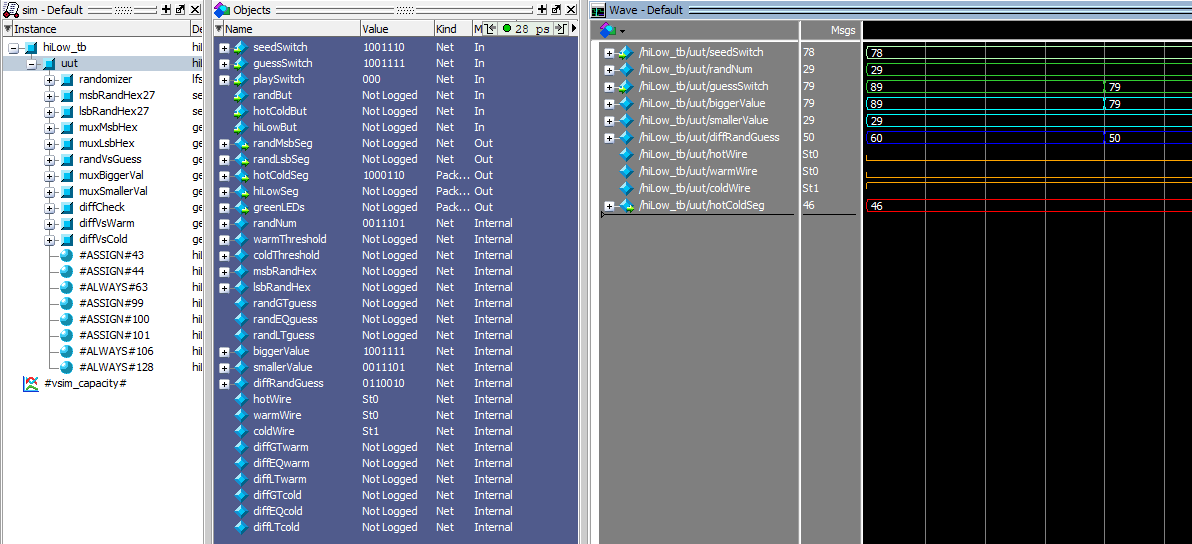
\includegraphics{ image6.png}
\caption{Use the design hierarchy to add signals to the testbench.}
\label{fig:hierarchyTestbench}
\end{figure}

When compete, your testbench should look like the timing diagram in
Figure~\ref{fig:guessTiming}.

\begin{figure}[ht]
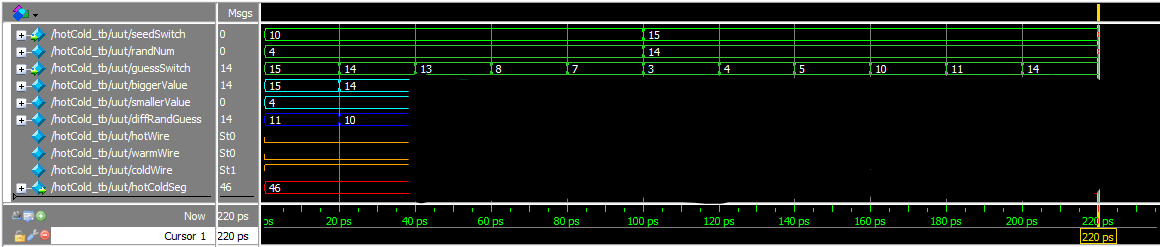
\includegraphics{ image7.png}
\caption{A partially obscured timing diagram generated by the testbench.}
\label{fig:guessTiming}
\end{figure}
\end{itemize}

\subsubsection{Demo}
\begin{itemize}
\item Demonstrate your completed circuit by the start of next week's lab.
\end{itemize}

\section{Debugging Tips}

When my program executed successfully, I got the warnings shown in
Figure~\ref{fig:messageConsole}. These are mainly the result of the unused overflow outputs
from the adder subtractor. You can filter out all the compile messages
by clicking on the yellow triangle (with the blue three in this case) on
the top line of the console window. Note, if there are several related
warnings, they will have one top-level warning with all the instances
accessible by clicking the expander arrow (it looks like
``\textgreater'') to the left of the warning triangle.

\begin{figure}[ht]
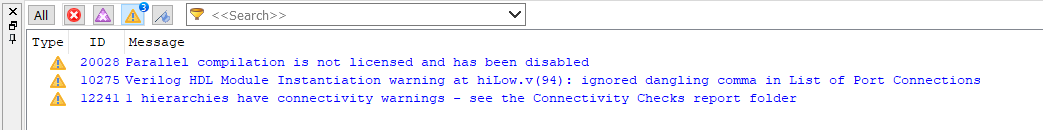
\includegraphics{image8.png}
\caption{The messages console filtered by warnings.}
\label{fig:messageConsole}
\end{figure}

I have found the Connectivity Checks folder in the Compilation Report to
help me quickly track down errors. To use it, open the Connectivity
Checks folder, click on a Port Connectivity Checks item and read the
report in the right pane. In the report shown in Figure~\ref{fig:connectivityCheck}, I selected
the genericAdderSubtractor and note I hardwired fnc to 1 so that it
always subtracts. This report also shows that the overflow outputs are
unconnected because we left them open using a pair of commas talked
about earlier.

\begin{figure}[ht]
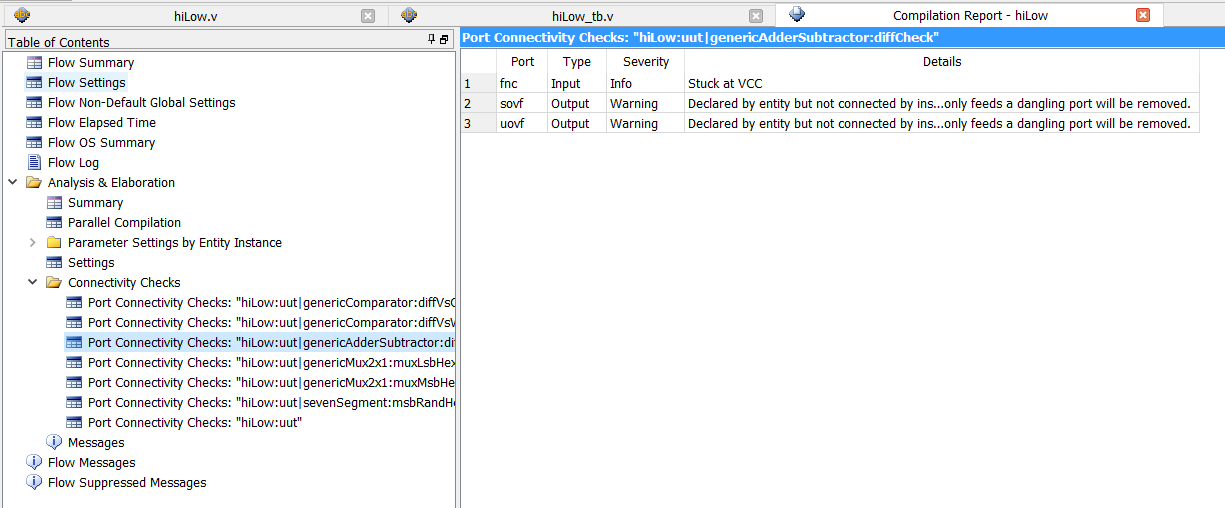
\includegraphics{ image9.png}
\caption{Connectivity Checks report for a working hiLow circuit.}
\label{fig:connectivityCheck}
\end{figure}

